\documentclass{article}

\usepackage{amsmath}
\usepackage{fancyhdr}
\usepackage{graphicx}
\graphicspath{{}}
\usepackage{placeins}
\usepackage{hyperref}
\usepackage[utf8]{inputenc}
\usepackage[margin=1in]{geometry}
\usepackage{titling}
\usepackage{datenumber}

\usepackage{minted}

%% some colours
\usepackage{xcolor}
\definecolor{deepblue}{rgb}{0,0,0.5}
\definecolor{deepred}{rgb}{0.6,0,0}
\definecolor{deepgreen}{rgb}{0,0.5,0}
\definecolor{backcolour}{rgb}{0.95,0.96,0.93}

%%%%%%%%%%%%%% CODE STUFF %%%%%%%%%%%%%%
%%%%%%%%%%%%%%%%%%%%%%%%%%%%%%%%%%%%%%%%
\newminted{python}{frame=single, framesep=5pt, linenos=true}
\newminted[outputcode]{text}{frame=single, framesep=5pt}


%%%%%%%%%%%%%%%%%%%%%%%%%%%%%%%%%%%%%%%%
% setting the style for ex documents
\pagestyle{fancy}
\fancyhf{}
\fancyhead[L]{\thetitle}
\fancyhead[C]{}
\fancyhead[R]{\theauthor}
\renewcommand{\headrulewidth}{0.4pt} %obere Trennlinie
\fancyfoot[L]{Due: \thedate}
\fancyfoot[R]{\thepage} %Seitennummer
\renewcommand{\footrulewidth}{0.4pt}

% include solutions
\ifdef{\solutions}
    {\newenvironment{solution}{\noindent \textbf{Solution:}}{}}
    % adapted from https://tex.stackexchange.com/a/194146
    {\newenvironment{solution}{\setbox0=\vbox\bgroup}{\egroup\iffalse\box0\fi}}


% Python execution environment
\newenvironment{pyexec}[1]{\noindent \textbf{Output: }  #1}{}


\author{K.\ Groß \and M.\ Pömsl \and S.\ Selbach}

\AtBeginDocument{
    \date{\datedate}
    The deadline for this exercise sheet is \textbf{\datedayname, \thedate\ at 23:59 CEST.}
}

\makeatletter
\tw@make@key@box{OS@mac}{\faApple}
\tw@make@key@box{OS@win}{\faWindows}
\tw@make@key@macro*{\OS}
\makeatother

\title{BPP Exercise 1 -- Introduction}
% {YYYY}{MM}{DD}
\setdate{2020}{04}{21}


\begin{document}

\section*{About the Exercise Sheets}

Normally all tasks on each exercise sheet will be graded. Since this is the first week, only the third and fourth task will be graded (but you need to complete the others in order to get everything set up). You can estimate how much time you should spend on each task by the points indicated in parentheses. To pass a sheet your solution should cover at least 60\% of the whole sheet.

\vspace{1em}

\noindent There will be 12 exercise sheets in total for this course. Each sheet you pass will earn you a homework point. You need at least 10 homework points to pass the course. There will also be the option for your group to submit a programming project worth 2-3 homework points.

\vspace{1em}

\noindent Please solve the sheets together as a group and hand in only one solution for each sheet. First save the solutions for each task in a separate file, then pack everything into a .zip archive. Finally upload your .zip file into your group folder on StudIP before the deadline.


\section{Installing Python}

To get started, we of course need to download and install the Python language. There are many, many flavours of Python, but for our purposes it mostly will not matter which one we choose. We will provide instructions on how to install Anaconda, which has some additional features that will come in handy if you want to pursue programming in Python further after this course. If for some reason you want an even lighter Python installation (e.g. less than 5GB or shitty internet connection), replace \textit{Anaconda} by \textit{Miniconda} in the following instructions.

\subsection{Opening a Terminal}

\vspace{1em}

\textbf{Windows:} Press \keys{\OS + R} and type \texttt{cmd} into the window that opens. Press \keys{\return}.

\vspace{1em}

\noindent \textbf{macOS:} Press \keys{\cmdmac + \Space} to open spotlight and type \texttt{terminal}. Then press \keys{\return}.

\vspace{1em}

\noindent \textbf{Ubuntu:} Press \keys{\ctrl + \Alt + T}.

\vspace{1em}

\subsection{Downloading Anaconda}

First, open your favourite browser, go to the Anaconda website \url{https://www.anaconda.com/products/individual} (for Miniconda: \url{https://docs.conda.io/en/latest/miniconda.html}) and download the appropriate installer for your operating system (you probably have a 64-bit system). On MacOS choose the Command Line Installer, On Linux the one just called Installer. Save the file someplace where you can find it again.

\subsection{Installing Anaconda}

\subsubsection*{For Windows Users:}

Find the installer you downloaded in 1.2 and double click it. You can accept the default options \textbf{except for the section "Advanced Options"}. Make sure both the box about the \texttt{PATH} variable and the box about the system's default Python are checked! Click on \keys{Install} and let the installer do its thing.

\subsubsection*{For Linux Users:}

Open a terminal, navigate to the installer you downloaded in 1.2, type \texttt{bash Anaconda3-2020.11-Linux-x86\_64.sh} and press \keys{\return}. Once again press the enter key and hold it until the User License Agreement has finished. If you agree, type \texttt{yes} and press enter. Once again press enter to confirm the location of the installation. After the installation has finished, once more type \texttt{yes} and press enter to confirm necessary additions to your \texttt{.bashrc} file.


\subsubsection*{For MacOS Users:}

Open a terminal, navigate to the installer you downloaded in 1.2, type \texttt{bash Anaconda3-2020.11-MacOSX-x86\_64.sh} and press \keys{\return}. Once again press the enter key and hold it until the User License Agreement has finished. If you agree, type \texttt{yes} and press enter. Once again press enter to confirm the location of the installation. After the installation has finished, once more type \texttt{yes}. For the changes to take effect, you have to close this terminal and open a new one.


\subsection{Testing your Installation}

To check whether everything is set up correctly, open a terminal.

\vspace{1em}

\noindent In the terminal, type \texttt{python} and press \keys{\return}. You should now see something like this:

\vspace{1em}

\noindent 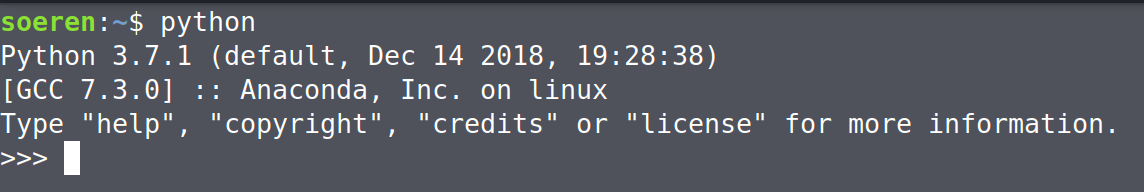
\includegraphics[width=\textwidth]{01_Introduction/python_shell.png}

\vspace{1em}

\noindent This is the Python shell. If for some reason it says \texttt{Python 2.x} instead of \texttt{Python 3.7}, you need to use the command \texttt{python3} instead of \texttt{python} for the remainder of this course.

\vspace{1em}

\noindent Type \texttt{import this} and see what happens!

\subsection{Installing Atom}

You have learned in the lecture that Python scripts are no more than simple text files. As such, you can use many different programs to edit them (but perhaps not \textit{all} the ones you think - Microsoft Word for instance is not a pure text editor!). We suggest you use \textbf{Atom} because it is simple to use and can be adapted to more complex needs as you progress in your programming life.

\vspace{1em}

\noindent You can download Atom from this website: \url{https://atom.io/}. The installation process should be straightforward. You can test whether it works by typing \texttt{atom} into the terminal.

\noindent For Windows users: In order to use Atom from the command prompt easily, you should add it to your PATH system variable (in MacOS and Linux this should happen automatically): 

\begin{itemize}
    \item In the control panel navigate to \textit{System->Advanced System Settings->Environment Variables}
    \item Under System Variables select PATH and click on edit
    \item At the end add ";C:\textbackslash Users\textbackslash \textit{Username}\textbackslash anaconda3\textbackslash condabin", where \textit{Username} is the username under which conda was installed. If you installed miniconda replace \textit{anaconda3}. If you installed anaconda in a different folder than the default one, you'll have to change what you add to PATH accordingly.

\end{itemize}

\section{Getting Used to the Terminal}

\subsection{Baby Steps}

First, open a terminal like you did in 1.3. Try to navigate to your desktop (the desktop is just another directory). There is a list of basic terminal commands on slide 22 of this week's lecture.

\vspace{1em}

\begin{solution}
    \begin{outputcode}
cd Desktop
    \end{outputcode}
\end{solution}

\noindent It is probably a good idea to have a dedicated directory for this course. On your desktop (or in any other place that you can find again), create a new directory called \texttt{BasicPython} using the terminal. What goes wrong if you try to name it \texttt{Basic Python} (with a space)?

\vspace{1em}
\begin{solution}
    \begin{outputcode}
mkdir BasicPython
    \end{outputcode}

    \noindent If there is a space between the words Basic and Python, \texttt{mkdir} will think you meant to create two distinct directories. However, you can still make it work like this:

    \begin{outputcode}
mkdir "Basic Python"
    \end{outputcode}

\end{solution}

\noindent Now create a directory called \texttt{Week01} \textbf{inside} your \texttt{BasicPython} directory.

\vspace{1em}

\begin{solution}
    \begin{outputcode}
cd BasicPython
mkdir Week01
    \end{outputcode}
\end{solution}

\subsection{Some New Commands}

Inside the \texttt{Week01} directory, run the command \texttt{atom my\_script.py}. This will create a new file \texttt{my\_script.py} and open it with Atom. Save the file and go back to the terminal.

\vspace{1em}

\noindent The next command you will use is \texttt{cp <file\_to\_copy> <destination\_of\_copy>}. Use it to create a copy of \texttt{my\_script.py}. Use \texttt{ls} or \texttt{dir} to show both files.

\vspace{1em}

\begin{solution}
    \begin{outputcode}
cp my_script.py my_script_copy.py
    \end{outputcode}
\end{solution}

\noindent Now use \texttt{rm <file\_to\_delete>} to delete the file \texttt{my\_script.py}. Did you notice there wasn't any warning or confirmation? The file also did not go to the trash folder, but was deleted permanently. You can do a lot of damage to your system with the terminal, so always double check what you type in.

\vspace{1em}

\begin{solution}
    \begin{outputcode}
rm my_script.py
    \end{outputcode}
\end{solution}

\noindent Lastly, there is \texttt{mv <old\_file> <new\_file>}. It moves a file from one location to another location. This can also be used to rename a file. Use it now to rename the copy you created before to \texttt{logo.py}.

\vspace{1em}

\begin{solution}
    \begin{outputcode}
mv my_script_copy.py logo.py
    \end{outputcode}
\end{solution}

\subsection{Using Auto-Complete}

You may have gotten the impression that using the terminal to create directories, copy files etc. looks very cool, but is slow compared to just doing it in a file explorer. However, once you practise a bit, you will actually be much quicker this way - and a big part of that is using auto-completion. Whenever you are typing a \textit{filename}, you can press \keys{\tab} after the first three letters or so. The terminal will then try to guess which file you meant, based on which files exist in the current working directory. Play around with this feature by for instance typing \texttt{cp dra} and then hitting \keys{\tab}.


\section{Basic Operations in the Python Shell}

For this task you have to open a Python shell by opening a terminal as described in 1.1. and then executing the command \texttt{python}. When you are done with the task, use atom to create a file named \texttt{operators.txt} and save your results in it (on line for each result).

\subsection{Operations on Numbers}

In the lecture you learned how the Python shell can be used like a text-based calculator. In this task we want you to make use of it. Using the Python shell and the operators \texttt+, \texttt-, \texttt*, \texttt/ and \texttt{**}, calculate the results of the following formulas:

\begin{enumerate}

\item $5 + 2 - 7$
\item $\frac{7}{5}$
\item $12 \cdot 274.3$
\item $2^{\frac{24}{7}}$
\item $\frac{3674 + 280398}{(3678 + 2321) * 43}$

\end{enumerate}

\begin{solution}
    \begin{outputcode}
0
1.4
3291.6000000000004
10.767201541058848
1.101237803199758
    \end{outputcode}
\end{solution}

\subsection{Operations on Text}

We also learned how the operators can be applied to text in quotation marks.
Which commands would you use to get the following outputs in the terminal?

\begin{enumerate}

\item How are you?
\item Hello! Hello! Hello! Hello!

\begin{solution}
    \begin{pythoncode}
print("How are you?")
print("Hello! " * 4)
    \end{pythoncode}
\end{solution}

\end{enumerate}

\subsection{Bonus Questions}

Why are the outputs of \texttt{print("7" + "9")} and \texttt{print(7 + 9)} different?

\vspace {1em}

\begin{solution}
    The \texttt{""} tell Python that \texttt{"7"} and \texttt{"9"} are to be treated as strings. The \texttt{+} operator on strings acts as a concatenation, while on numbers it acts as addition.
\end{solution}

\vspace{1em}

\noindent What is the difference between \texttt{print(7 / 9)} and \texttt{print(7 // 9)}?

\begin{solution}
    \texttt{/} is the "normal" division operator which can have floating point numbers as output. \texttt{//} is called the \textit{integer division} operator because it always rounds the result down to the next integer.
\end{solution}

\section{Turtle!}

For this task open a Python shell once again and execute the following commands:

\begin{pythoncode}

from turtle import forward, right, left, penup, pendown, reset
forward(0)

\end{pythoncode}

\noindent You should see a turtle now! Or at the very least a moving arrow. Try moving it with the command \texttt{forward(100)}.
With \texttt{reset()}, you can set it back to its initial position. What happens if you do just \texttt{forward(50)} instead of \texttt{forward(100)}?
\texttt{right(90)} and \texttt{left(90)} will make the turtle turn around. \texttt{penup()} and \texttt{pendown()} influence whether the turtle will draw a line when walking or not. Try experimenting with the other commands as well!

\vspace{1em}

\noindent In the lecture you have learned that Python code can not only be executed in a Python terminal step by step, but also from a \texttt{.py} file - a so called script. Your task is to write a script that will open the turtle window and make it draw a logo for your group. This logo can be anything, depending on your creativity and motivation. It could be a word, an animal, a plant - whatever you like.

\vspace{1em}

\noindent Use atom to create this script and save it as \texttt{logo.py}. Then try executing it from the terminal with the command \texttt{python logo.py}. This should be handed in as well, so your solution for this exercise sheet should consist of a .zip file containing the file \texttt{operators.txt} from task 3 as well as \texttt{logo.py}.

\noindent Below you can find an example of how a script to write the letter "M" could look like:

\begin{pythoncode}

from turtle import forward, right, left, penup, pendown, reset

penup()
right(180)
forward(100)
pendown()
right(90)
forward(150)
right(150)
forward(100)
left(120)
forward(100)
right(150)
forward(150)

input()

\end{pythoncode}

\noindent You can ignore the \texttt{input()} for now, it is just there to make the script wait for you to press a key until the window closes. Now go on and train your own turtle!

\newpage

\section*{Afterword}

\noindent We always try to structure the exercise sheets so that all concepts you need will already have been explained in the lecture. If despite that we ask for something that you have no idea how to do, try the following steps in this order:

\begin{enumerate}

\item Check the relevant lecture slides (including the grey notes) and the whole exercise sheet.
\item Use your favourite search engine on relevant keywords in conjunction with "python 3".
\item If you did not find anything on the internet, come to the practice session on Thursday.
\item If you can't make it to the practice session, send us a mail explaining your problem and how you tried to solve it so far.

\end{enumerate}

\vspace{1em}

\noindent We wish you all the best for the first exercise sheet!

\vspace{1em}

\noindent Jonas (jkraasch@uos.de) and Johanna (jtamm@uos.de)



\end{document}
